\documentclass[11pt,a4paper]{article}
\usepackage[utf8]{inputenc}
\usepackage[T1]{fontenc}
\IfFileExists{french.ldf}{\usepackage[french]{babel}}{\usepackage[english]{babel}}
\usepackage{amsmath,amssymb,amsthm}
\usepackage[margin=2.3cm]{geometry}
\usepackage{listings}
\usepackage{xcolor}
\usepackage{enumitem}
\usepackage{tikz}
\usepackage{hyperref}
\hypersetup{colorlinks=true, urlcolor=[RGB]{2,101,115}, linkcolor=black, citecolor=black}
\definecolor{codebg}{RGB}{247,249,251}
\definecolor{kw}{RGB}{175,45,45}
\definecolor{cmt}{RGB}{110,120,130}
\definecolor{str}{RGB}{20,110,60}
\lstset{language=Python, backgroundcolor=\color{codebg}, basicstyle=\ttfamily\small,
  keywordstyle=\color{kw}\bfseries, commentstyle=\color{cmt}\itshape, frame=single,
  rulecolor=\color{gray!40}, columns=fullflexible, breaklines=true, showstringspaces=false,
  aboveskip=5pt, belowskip=5pt, extendedchars=true, inputencoding=utf8,
  literate={é}{{\'e}}1 {è}{{\`e}}1 {à}{{\`a}}1 {ê}{{\^e}}1 {î}{{\^i}}1 {ç}{{\c c}}1 {ô}{{\^o}}1 {É}{{\'E}}1}
\newcommand{\code}[1]{\lstinline!#1!}
\theoremstyle{definition}\newtheorem{definition}{Définition}
\theoremstyle{plain}\newtheorem{theoreme}{Théorème}\newtheorem{proposition}{Proposition}
\theoremstyle{remark}\newtheorem{remarque}{Remarque}
\renewcommand{\proofname}{Démonstration}
\setlength{\parskip}{0.35em}

\begin{document}

\begin{center}
{\large\bfseries Agrégation externe d'informatique}\\[3pt]
{\bfseries Épreuve de modélisation}\\[10pt]
\rule{0.85\linewidth}{0.4pt}\\[8pt]
{\LARGE\bfseries Arbres de Merkle et vérification légère\\[2pt] dans Bitcoin}\\[8pt]
\rule{0.85\linewidth}{0.4pt}
\end{center}

\medskip
\begin{center}
\fbox{\begin{minipage}{0.95\linewidth}\small
Il est rappelé que le jury n'exige pas une compréhension exhaustive du texte. Vous êtes
laissé(e) libre d'organiser votre présentation comme vous l'entendez. Il vous est conseillé de
mettre en valeur vos connaissances et votre culture scientifique à partir du fil conducteur
constitué par le texte. Les \emph{suggestions de développement}, en fin de texte, ne sont là que
pour vous aider~; vous ne devez pas vous sentir tenu(e) de les suivre, ni de les traiter toutes.
Le jury appréciera que votre exposé s'accompagne d'\textbf{exemples, d'implémentations et
d'expériences} menés sur ordinateur (Python conseillé~: \texttt{hashlib}, \texttt{numpy},
\texttt{matplotlib}).
\end{minipage}}
\end{center}

\bigskip
\section{Le problème : vérifier sans tout télécharger}

Une chaîne de blocs de type Bitcoin est répliquée sur des milliers de machines indépendantes~;
sa taille se compte en centaines de gigaoctets. Un utilisateur muni d'un simple téléphone ne peut
ni stocker ni revalider l'intégralité de l'historique. Pourtant, il souhaite s'assurer qu'une
transaction précise --- par exemple un paiement qui le concerne --- a bien été incluse dans un
bloc accepté par le réseau. Le problème central est donc celui d'une \emph{vérification légère}~:
convaincre un client de faible capacité de l'\emph{appartenance} d'une donnée à un très grand
ensemble, à l'aide d'un \emph{certificat} de taille minimale, sans lui transmettre l'ensemble
entier ni exiger qu'il le recalcule.

La solution retenue par Bitcoin (S.~Nakamoto, 2008), et devenue un standard, repose sur une
structure de données \emph{authentifiée}~: l'\emph{arbre de Merkle} (R.~Merkle, 1979). Le fil
conducteur de ce texte relie une brique cryptographique (la fonction de hachage), une structure
arborescente et sa complexité, une preuve de correction fondée sur une \emph{réduction}, et enfin
un modèle probabiliste de la \emph{preuve de travail} qui sécurise l'ajout des blocs. Chaque
notion se prête à une implémentation et à une expérimentation numérique.

\section{Hachage cryptographique et collisions}

Bitcoin identifie chaque objet par son \emph{double SHA-256}
\[
  H(m) = \mathrm{SHA256}\bigl(\mathrm{SHA256}(m)\bigr) \in \{0,1\}^{256},
\]
que l'on peut voir comme une application $H:\{0,1\}^{*}\to\{0,1\}^{256}$. Une transaction $t$ est
résumée par son identifiant $\mathrm{txid}=H(t)$. Deux propriétés opposées coexistent.

\begin{proposition}[Existence des collisions]\label{prop:tiroirs}
L'application $H$ n'est pas injective~: il existe des messages distincts de même haché.
\end{proposition}
\begin{proof}
L'ensemble de départ est infini, l'ensemble d'arrivée fini (de cardinal $2^{256}$)~; par le
principe des tiroirs, $H$ ne peut être injective.
\end{proof}

Les collisions existent donc, mais on postule qu'elles sont \emph{introuvables en pratique}~: il
n'existe pas d'algorithme efficace produisant $m\neq m'$ avec $H(m)=H(m')$. Cette \emph{résistance
aux collisions} est une hypothèse \emph{calculatoire}, et non un théorème. Sa force se mesure par
l'attaque générique la plus simple, que le modèle de l'\emph{oracle aléatoire} permet d'analyser.

\begin{proposition}[Borne des anniversaires]\label{prop:birthday}
En tirant $k$ valeurs indépendantes et uniformes parmi $M=2^{b}$, la probabilité d'\emph{absence}
de collision vaut $q_k=\prod_{i=0}^{k-1}(1-i/M)$ et vérifie
$q_k\le \exp\!\bigl(-k(k-1)/2M\bigr)$. Une collision devient probable dès que
$k\gtrsim 1{,}177\,\sqrt{M}=1{,}177\cdot 2^{b/2}$.
\end{proposition}
\begin{proof}
Le $i$-ième tirage évite les $i$ valeurs déjà obtenues avec probabilité $1-i/M$~; par
indépendance on obtient le produit. L'inégalité $1-x\le e^{-x}$ donne
$q_k\le \exp(-\sum_{i<k} i/M)=\exp(-k(k-1)/2M)$, quantité $\le 1/2$ dès que $k(k-1)\ge 2M\ln 2$.
\end{proof}

Ainsi une empreinte sur $b$ bits n'offre qu'une résistance de l'ordre de $2^{b/2}$ opérations~:
le choix $b=256$ vise une marge de $2^{128}$, hors de portée. Le cas $M=365$ n'est autre que le
célèbre \emph{paradoxe des anniversaires} ($23$ personnes suffisent). Ces seuils s'observent
aisément par une expérience de Monte-Carlo sur une empreinte tronquée à $b$ bits.

\begin{lstlisting}
import hashlib, random
def H(m: bytes) -> bytes:
    return hashlib.sha256(hashlib.sha256(m).digest()).digest()
def tronque(h: bytes, b: int) -> int:      # b premiers bits de h
    return int.from_bytes(h, "big") >> (256 - b)
# On peut mesurer le nombre de tirages avant la premiere collision, pour b=16,24,32,
# et le comparer a l'ordre de grandeur 2^{b/2} predit par la Proposition 2.
\end{lstlisting}

\section{L'arbre de Merkle d'un bloc}

Un bloc contient une liste ordonnée de transactions $t_0,\dots,t_{n-1}$. On les résume en un
unique haché, la \emph{racine de Merkle}, placé dans l'en-tête du bloc. La construction procède
par niveaux~: partant des feuilles $\mathrm{txid}_i=H(t_i)$, on remplace chaque paire consécutive
$(a,b)$ par $H(a\Vert b)$ (concaténation des octets)~; \emph{si un niveau contient un nombre impair
de n\oe uds, on duplique son dernier élément} avant l'appariement (règle propre à Bitcoin). On
itère jusqu'à obtenir un seul haché.

\begin{center}
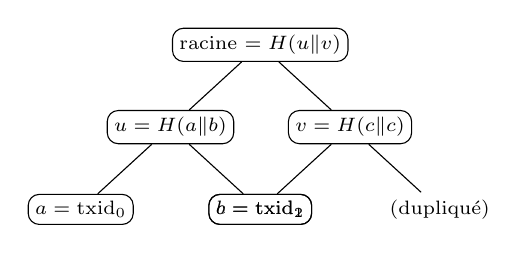
\begin{tikzpicture}[level distance=11mm, sibling distance=24mm, scale=0.95,
  every node/.style={draw,rounded corners,inner sep=2.5pt,font=\scriptsize,minimum width=13mm}]
\node {racine $=H(u\Vert v)$}
  child {node {$u=H(a\Vert b)$} child {node {$a=\mathrm{txid}_0$}} child {node {$b=\mathrm{txid}_1$}}}
  child {node {$v=H(c\Vert c)$} child {node {$c=\mathrm{txid}_2$}} child[draw=none] {node[draw=none]{\scriptsize(dupliqué)}}};
\end{tikzpicture}\\[-1pt]
{\footnotesize Figure~1 --- arbre de Merkle d'un bloc à trois transactions~: le dernier haché est dupliqué.}
\end{center}

\begin{proposition}[Coût de construction]\label{prop:cout}
Le calcul de la racine de $n$ transactions demande $O(n)$ évaluations de $H$, en temps et espace
$O(n)$, et l'arbre a une hauteur $\lceil\log_2 n\rceil$.
\end{proposition}
\begin{proof}
En notant $t_0=n$ et $t_{k+1}=\lceil t_k/2\rceil$ la taille du niveau $k+1$, on a
$t_{k+1}\le t_k/2+1$, d'où $t_k\le n2^{-k}+2$~: la hauteur est $\lceil\log_2 n\rceil$ et il y a
$O(\log n)$ niveaux. Le total des évaluations vaut $\sum_{k\ge1} t_k\le n+O(\log n)=O(n)$.
\end{proof}

\begin{remarque}[Une subtilité de sécurité]\label{rem:cve}
La règle de duplication a une conséquence inattendue~: pour certains $n$, un bloc et un bloc
obtenu en dupliquant réellement des transactions produisent la \emph{même} racine. Cette
ambiguïté (connue sous le nom de \guillemotleft~CVE-2012-2459~\guillemotright) illustre qu'une
structure authentifiée doit être analysée avec soin~: la racine seule ne garantit pas l'unicité de
l'arbre sous-jacent.
\end{remarque}

\section{Preuves d'inclusion et clients légers (SPV)}

Un client \emph{léger} (\emph{Simplified Payment Verification}) ne conserve que les en-têtes des
blocs, donc les racines. Pour lui prouver qu'une transaction $t$ appartient à un bloc de racine
$R$, on lui fournit une \emph{preuve de Merkle}~: la suite des hachés \emph{frères} rencontrés en
remontant de la feuille $H(t)$ jusqu'à la racine, chacun accompagné de son côté (gauche ou
droite). Le client recombine ces hachés par $H$ et accepte si et seulement s'il retrouve $R$.

La longueur d'une telle preuve est le nombre de niveaux, soit $\lceil\log_2 n\rceil=O(\log n)$~:
pour un bloc de dizaines de milliers de transactions, une poignée de hachés suffit, là où le
téléchargement du bloc entier serait prohibitif. C'est précisément ce qui rend le modèle SPV
viable sur un appareil modeste. La \emph{sûreté} de ce mécanisme se ramène à la seule hypothèse
sur $H$.

\begin{theoreme}[Sûreté de la vérification, ou \emph{soundness}]\label{th:soundness}
Supposons $H$ résistante aux collisions. Si la vérification d'une preuve d'inclusion pour une
valeur $x$ aboutit à la racine authentique $R$, alors --- sauf à exhiber une collision de $H$ ---
la valeur $x$ figure réellement parmi les transactions ayant produit $R$.
\end{theoreme}
\begin{proof}
Récurrence sur la hauteur $H$ de l'arbre. Si $H=0$, la racine \emph{est} la feuille et la preuve
est vide~: l'acceptation impose $x=R$. Hérédité~: la vérification calcule d'abord
$r'=H(x\Vert f)$ (ou $H(f\Vert x)$) avec le premier frère $f$, puis poursuit~: c'est une preuve
d'inclusion valide de $r'$ dans l'arbre de hauteur $H$ des n\oe uds du niveau supérieur. Par
hypothèse de récurrence, ou bien $r'$ est un n\oe ud authentique de ce niveau, ou bien on a
produit une collision. Dans le premier cas, $r'$ possède déjà un antécédent authentique par $H$
issu de la construction~; l'égalité $H(x\Vert f)=r'$ fournit soit ce même couple (et alors $x$ est
la feuille attendue), soit un couple distinct de même image, c'est-à-dire une collision de $H$.
En l'absence de collision calculable, $x$ appartient donc bien au bloc.
\end{proof}

\begin{remarque}
La sécurité de tout l'édifice se \emph{réduit} ainsi à celle de $H$~: forger une fausse preuve
d'inclusion revient à calculer une collision (Proposition~\ref{prop:birthday}). Cette réduction
est la véritable justification du dimensionnement $b=256$.
\end{remarque}

\section{La preuve de travail : un modèle probabiliste}

Rester léger suppose de faire confiance à la chaîne d'en-têtes reçue. Bitcoin rend cette chaîne
coûteuse à falsifier par la \emph{preuve de travail}. L'en-tête d'un bloc contient un entier
libre, le \emph{nonce} $\nu$~; \emph{miner} le bloc, c'est trouver $\nu$ tel que $H(e_\nu)$,
interprété comme un entier sur $256$ bits, soit inférieur à une \emph{cible} $T$. Dans le modèle
de l'oracle aléatoire, chaque essai réussit indépendamment avec probabilité $p=T/2^{256}$.

\begin{proposition}[Coût du minage]\label{prop:pow}
Le nombre $N$ d'essais jusqu'au premier succès suit une loi géométrique de paramètre $p$~; son
espérance est $\mathbb{E}[N]=1/p$, et le minage \emph{termine presque sûrement}
($\mathbb{P}(N=\infty)=\lim_k (1-p)^{k}=0$).
\end{proposition}

Le minage est donc un algorithme \emph{probabiliste} de type Las~Vegas~: il rend toujours un
résultat correct, mais son temps d'exécution est aléatoire, d'espérance $1/p$. En pratique, on
fixe la difficulté en exigeant que le haché commence par $k$ bits nuls, soit $p=2^{-k}$ et
$\mathbb{E}[N]=2^{k}$~; la distribution de $N$ et cette espérance s'observent directement par
simulation. Le réseau ajuste périodiquement $T$ pour maintenir un intervalle moyen constant entre
blocs malgré la variation de la puissance de calcul.

\begin{lstlisting}
import itertools
def mine(entete: bytes, k: int) -> tuple[int, bytes]:
    for nu in itertools.count():
        h = H(entete + nu.to_bytes(4, "big"))
        if int.from_bytes(h, "big") >> (256 - k) == 0:   # k bits de tete nuls
            return nu, h
# En repetant le minage, on peut estimer E[N] et tracer l'histogramme de N (loi geometrique).
\end{lstlisting}

Enfin, la \emph{sécurité} de la chaîne se lit comme une course~: un attaquant de puissance
relative $\alpha<1/2$, parti avec $z$ blocs de retard, ne rattrape la chaîne honnête qu'avec une
probabilité qui \emph{décroît exponentiellement} en $z$. C'est ce qui fonde la règle des
\emph{confirmations} (attendre plusieurs blocs avant de tenir un paiement pour définitif), et ce
qui relie la vérification légère du client SPV à la robustesse économique du consensus.

\section{Prolongements et structures voisines}

L'arbre de Merkle binaire de Bitcoin admet de nombreuses variantes. Ethereum emploie un arbre de
\emph{Patricia-Merkle} (mêlant arbre préfixe et hachage) pour indexer un état modifiable~; les
\emph{arbres de Verkle} remplacent le hachage par des \emph{engagements polynomiaux} et abaissent
la taille des preuves de $O(\log n)$ à $O(1)$. Plus généralement, la vérification \guillemotleft~à
faible coût~\guillemotright{} illustrée ici est l'idée directrice des \emph{preuves à divulgation
nulle} et des \emph{rollups}~: déléguer un calcul massif tout en n'en vérifiant qu'un certificat.

\section*{Suggestions pour le développement}

\emph{Les pistes suivantes, largement indépendantes, ne sont qu'indicatives~; on n'en traitera
qu'une partie, en privilégiant celles que l'on peut à la fois exposer, illustrer par une
implémentation et éprouver par une simulation.}

\begin{itemize}[nosep,leftmargin=1.3em]
  \item Modéliser et implémenter la construction de la racine de Merkle d'un bloc, la génération
        et la vérification des preuves d'inclusion~; mettre en évidence expérimentalement la
        croissance logarithmique de la taille des certificats.
  \item Étudier la Proposition~\ref{prop:birthday}, en discuter l'équivalent asymptotique et la
        confronter à une expérience de Monte-Carlo sur une empreinte tronquée~; en déduire une
        interprétation du dimensionnement à $256$ bits.
  \item Analyser en détail le Théorème~\ref{th:soundness} et expliciter la \emph{réduction}~:
        comment une fausse preuve fournit-elle, de manière effective, une collision~?
  \item Approfondir la Remarque~\ref{rem:cve}~: caractériser les tailles de blocs sensibles à
        l'ambiguïté de la duplication et proposer une parade (vérification du nombre de feuilles).
  \item Étudier le modèle probabiliste du minage (Proposition~\ref{prop:pow})~: distribution de
        $N$, effet de l'ajustement de la cible, temps moyen entre blocs pour une puissance donnée.
  \item Simuler la \guillemotleft~course entre chaînes~\guillemotright{} et estimer la probabilité
        de rattrapage en fonction de $\alpha$ et $z$~; relier au choix du nombre de confirmations.
  \item Comparer, du point de vue de la complexité et de la taille des preuves, l'arbre binaire de
        Bitcoin, un arbre $k$-aire, l'arbre de Patricia-Merkle et les engagements de type Verkle.
  \item Situer la résistance aux collisions dans le cadre des \emph{fonctions à sens unique} et de
        la cryptographie à sécurité prouvée.
\end{itemize}

\section*{Références}
\begin{enumerate}[nosep,leftmargin=1.6em]
  \item S.~Nakamoto, \emph{Bitcoin: A Peer-to-Peer Electronic Cash System}, 2008.
  \item R.~C.~Merkle, \emph{A digital signature based on a conventional encryption function},
        CRYPTO~'87.
  \item A.~M.~Antonopoulos, \emph{Mastering Bitcoin}, O'Reilly~; A.~M.~Antonopoulos, G.~Wood,
        \emph{Mastering Ethereum}, O'Reilly.
  \item J.~Katz, Y.~Lindell, \emph{Introduction to Modern Cryptography}, CRC Press.
\end{enumerate}

\vfill
\noindent\rule{\linewidth}{0.3pt}\\
{\footnotesize\itshape Texte de modélisation proposé dans le cadre d'une préparation à
l'agrégation d'informatique par Pr Agrégé El Hadiq Zouhair --- \href{https://cpgeacademy.org}{cpgeacademy.org}.}

\end{document}
